\documentclass[a4paper, 10pt]{article}
\usepackage[utf8]{inputenc}
%\usepackage[brazil]{babel}
\usepackage[top=3cm,left=3cm,right=2cm,bottom=2cm]{geometry} % para as margens
\usepackage{graphicx} % para as figuras  
\usepackage{color}
\usepackage[hidelinks]{hyperref}
\usepackage{listings}

\newcommand{\ee}{CHOReOS Enactment Engine}


\title{\ee\ REST API}
\author{Leonardo Leite (IME - USP)}

\begin{document}

\maketitle

\section{Introduction}

This document provides detailed information about the \ee\ REST API. 
Understanding the API enables you to write your own code to enact a choreography.
Although the CHOReOS Dynamic Development Process automates the \ee\ invocation at the end of the Synthesis Process, writing your own client may be a good idea when you already have designed the choreography at the service interaction level and have chosen the concrete services. 

This document is organized as follows. Section \ref{sec:model} presents the data model that defines XML representations exchanged by API messages. Section \ref{sec:api} describes all the operations provided by the REST API, detailing parameters and return structures. Section \ref{sec:client} presents our client implementation that can be used within any Java program.

\section{Data model}
\label{sec:model}

As in any API, \ee\ operations receive and return complex data structures representing real world concepts. 
Figure \ref{img:data_model} presents these concepts in the UML notation.
Although the REST API handles XML representations, we use here the UML notation, since it makes easier to the reader to understand the concepts.

\begin{figure}
\centering
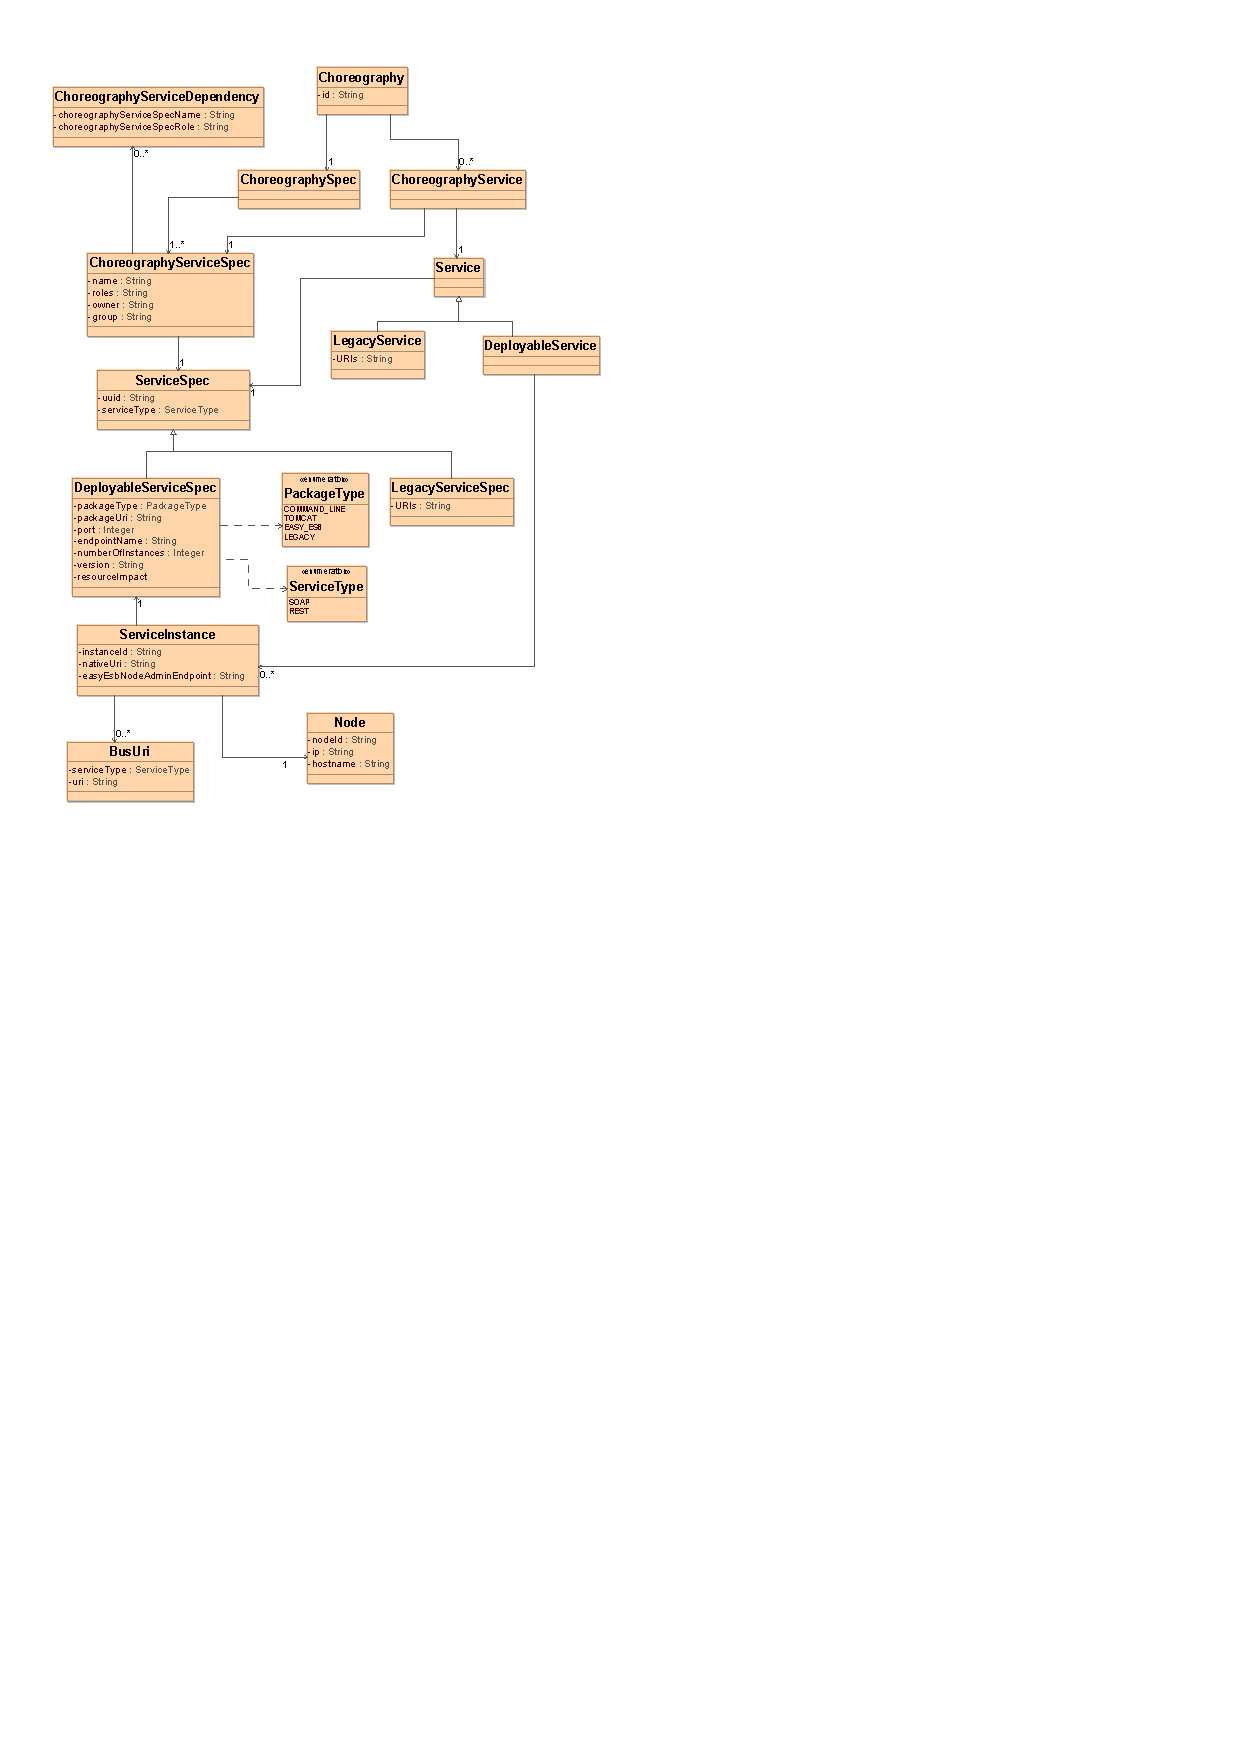
\includegraphics[scale=0.75]{img/data_model.pdf}
\caption{\ee\ REST API data model}
\label{img:data_model}
\end{figure}

We proceed with a brief explanation about each class:

\begin{description}
\item [ChorSpec:] represents what the middleware needs to know to enact a choreography;
\item [ServiceSpec:] represents what the middleware needs to know to deploy a service (with one or more instances for load balancing).
\item [ServiceDependency:] represents dependencies among services (if \verb!service A! invokes \verb!service B!, we say \verb!service A! depends on \verb!service B!);
\item [Choreography:] provides information about a choreography instance; 
\item [Service:] provides information about a deployed service. 
\item [ServiceInstance:] provides information about a specific instance, or replica, of a deployed service. 
\end{description}

To request a choreography enactment, it is important to understand very well the \verb!ServiceSpec! class. Therefore, the description of each one of its attributes follows:

\begin{description}
\item [name:] a unique name within the choreography specification;
\item [owner:] the organization that holds the infrastructure where the service must be deployed (not implemented, for now a single cloud per \ee\ instance is supported);
\item [group:] services in the same group will be deployed in the same cloud node (not implemented);
\item [roles:] list of roles implemented by the service;
\item [dependencies:] list of \verb!ServiceDependency! entries; each entry describes the name of the dependency (matching the \verb!name! attribute), and the the role provided by the dependency;
\item [type:] whether the service is a SOAP service or a REST service. More types can be added as necessary.
\item [packageType:] the type of the deployable artifact, according to the \verb!PackageType! enumeration\footnote{When the package type is COMMAND\_LINE the service will be executed by the ``java -jar'' command.};
\item [packageUri:] the location of the binary file to be deployed. If type is LEGACY (services that are not being deployed specifically for this choreography, but are already available somewhere), this attribute will represent the complete service endpoint;
\item [port:] the TCP port used by the service. Note that multiple replicas of a single service will all use the same port. Mandatory if type is COMMAND\_LINE;
\item [endpointName:] the endpoint suffix after deployment. For example, if the service will be deployed as \verb!http://<some_ip>/choreos/service!, the endpoint is \verb!choreos/service!. Note that multiple replicas of a single service will all use the same endpoint. If type is LEGACY, endpoint is empty.
\item [version:] the service version, which is used by the \ee\ to define which services must be redeployed in a choreography update.
\item [numberOfInstances:] How many instances of the service should be deployed (onto different virtual machines) in order to allow the load to be distributed.
\end{description}


\subsubsection*{More about dependencies}

In a service composition, some services depends on other services. A service that depends on other services is a \emph{consumer} service, and the service that provides functionality to the dependent service is the \emph{provider}. In simple service compositions, such dependency relations are hardcoded on consumer services. But decoupling the consumer service implementation from the actual provider endpoint is a good practice, which enables dynamic adaptation. Moreover, dependency hardcoding is not possible on cloud environments, since we do not know service addresses before deployment. Therefore, in the CHOReOS environment each consumer service is declared as depending on \emph{roles} rather than other service implementations. The consumer service must receive the actual provider endpoint of a service fulfilling the required role through the \verb!setInvocationAddress! operation, which every consumer service must implement.  

The \ee\ will use \verb!ServiceDependency! data to know which calls it must perform to the  \verb!setInvocationAddress! operation of participant services. Thus, the \ee\ will be able to tell, for example, to \verb!ServiceA! that it must use \verb!ServiceB! as \verb!Role1!, where \verb!ServiceB! is the list of endpoint URIs corresponding to the multiple instances of \verb!ServiceB!. In this way, the CHOReOS middleware provides a \emph{dependency injection}\footnote{Dependency Injection pattern, by Martin Fowler: \url{http://martinfowler.com/articles/injection.html}} mechanism to wire up service dependencies.

\subsubsection*{Resource impact specification}

The \verb!ServiceSpec! class has also an attribute to specify non-functional requirements, such as QoS constraints. This attribute is called ``resource impact'', and it can be used by the \verb!NodeSelector!\footnote{See the lesson Choreography Enactment.} to choose the node in which the service should be deployed. \verb!NodeSelector! will try to choose a node that enables the service to fulfil such requirements.

This attribute is not described in this document because its structure is not fully defined yet. But it is expected to define, among others, required values of CPU, memory, and disk usage.

\subsubsection*{XML representation}

Each class is mapped to and from an XML representation according to the default behaviour of the JAXB API\footnote{Java Architecture for XML Binding (JAXB): allows Java developers to map Java classes to XML representations.}. 
To properly build and read these XML representations, you can rely on the schema definition (XSD file) located in the appendix of this document. We provide here an example of \verb!ChorSpec! (Listing \ref{lst:chor_spec_xml}) and \verb!Choreography! (Listing \ref{lst:chor_xml}) XML representations to a little choreography with just two services (airline and travel-agency services). 

{\footnotesize

\lstset{language=XML}

\begin{lstlisting}[caption=ChorSpec XML representation example, label=lst:chor_spec_xml]
<chorSpec>
    <serviceSpecs>
        <endpointName>airline</endpointName>
        <name>airline</name>
        <numberOfInstances>1</numberOfInstances>
        <packageType>COMMAND_LINE</packageType>
        <packageUri>http://valinhos.ime.usp.br:54080/airline.jar</packageUri>
        <port>1234</port>
        <roles>airline</roles>
        <type>SOAP</type>
    </serviceSpecs>
    <serviceSpecs>
        <dependencies>
            <serviceName>airline</serviceName>
            <serviceRole>airline</serviceRole>
        </dependencies>
        <endpointName>travelagency</endpointName>
        <name>travelagency</name>
        <numberOfInstances>1</numberOfInstances>
        <packageType>COMMAND_LINE</packageType>
        <packageUri>http://valinhos.ime.usp.br:54080/travel.jar</packageUri>
        <port>1235</port>
        <roles>travelagency</roles>
        <type>SOAP</type>
    </serviceSpecs>
</chorSpec>\end{lstlisting}

\begin{lstlisting}[caption=Choreography XML representation example, label=lst:chor_xml]
<choreography>
    <deployedServices>
        <instances>
            <myParentServiceSpec>
                <endpointName>airline</endpointName>
                <name>airline</name>
                <numberOfInstances>1</numberOfInstances>
                <packageType>COMMAND_LINE</packageType>
                <packageUri>http://valinhos.ime.usp.br:54080/airline.jar</packageUri>
                <port>1234</port>
                <roles>airline</roles>
                <type>SOAP</type>
            </myParentServiceSpec>
            <nativeUri>http://192.168.56.101:1234/airline/</nativeUri>
            <node>
                <hostname>choreos-node</hostname>
                <id>1</id>
                <ip>192.168.56.101</ip>
            </node>
        </instances>
        <name>airline</name>
        <spec>
            <endpointName>airline</endpointName>
            <name>airline</name>
            <numberOfInstances>1</numberOfInstances>
            <packageType>COMMAND_LINE</packageType>
            <packageUri>http://valinhos.ime.usp.br:54080/airline.jar</packageUri>
            <port>1234</port>
            <roles>airline</roles>
            <type>SOAP</type>
        </spec>
    </deployedServices>
    <deployedServices>
        <instances>
            <myParentServiceSpec>
                <dependencies>
                    <serviceName>airline</serviceName>
                    <serviceRole>airline</serviceRole>
                </dependencies>
                <endpointName>travelagency</endpointName>
                <name>travelagency</name>
                <numberOfInstances>1</numberOfInstances>
                <packageType>COMMAND_LINE</packageType>
                <packageUri>http://valinhos.ime.usp.br:54080/travel.jar</packageUri>
                <port>1235</port>
                <roles>travelagency</roles>
                <type>SOAP</type>
            </myParentServiceSpec>
            <nativeUri>http://192.168.56.102:1235/travelagency/</nativeUri>
            <node>
                <hostname>choreos-node</hostname>
                <id>2</id>
                <ip>192.168.56.102</ip>
            </node>
        </instances>
        <name>travelagency</name>
        <spec>
            <dependencies>
                <serviceName>airline</serviceName>
                <serviceRole>airline</serviceRole>
            </dependencies>
            <endpointName>travelagency</endpointName>
            <name>travelagency</name>
            <numberOfInstances>1</numberOfInstances>
            <packageType>COMMAND_LINE</packageType>
            <packageUri>http://valinhos.ime.usp.br:54080/travel.jar</packageUri>
            <port>1235</port>
            <roles>travelagency</roles>
            <type>SOAP</type>
        </spec>
    </deployedServices>
    <id>1</id>
</choreography>
\end{lstlisting}

}

\section{REST API}
\label{sec:api}

The \ee\ clients access its features though a REST API exposed by the Choreography Deployer component. This API is described in this section.

\subsubsection*{Create a choreography}

\begin{tabular}{|c|c|c|c|}
\hline 
\itshape{HTTP Method} & \itshape{URI} & \itshape{Request body} & \itshape{Responses} \\ 
\hline 
POST & /chors & 

\begin{minipage}{2in}
\verb!ChorSpec! XML representation \\ 
(see Listing \ref{lst:chor_spec_xml})
\end{minipage} 
&

\begin{minipage}{2in}
\begin{verbatim}

201 CREATED
location = "/chors/{id}"

400 BAD REQUEST

500 ERROR

\end{verbatim}
\end{minipage} 
\\ 
\hline 
\end{tabular} \\

Creates a specification of the choreography on the \ee.
It does not enact the choreography. \\

\subsubsection*{Retrieve choreography information}

\begin{tabular}{|c|c|c|c|}
\hline 
\itshape{HTTP Method} & \itshape{URI} & \itshape{Request body} & \itshape{Responses} \\ 
\hline 
GET & /chors/\{id\} & - &
\begin{minipage}{2in}
\begin{verbatim}

200 OK
location = "/chors/{id}"

Body: 
\end{verbatim}
\verb!Choreography! XML \\
representation \\
(see Listing \ref{lst:chor_xml})
\begin{verbatim}
400 BAD REQUEST

404 NOT FOUND

500 ERROR

\end{verbatim}
\end{minipage} 
\\ 
\hline 
\end{tabular} \\

If this operation is invoked after the creation and before the enactment of a choreography, the body response will be a \verb!Choreography! representation without any deployed service.

\subsubsection*{Enact a choreography}

\begin{tabular}{|c|c|c|c|}
\hline 
\itshape{HTTP Method} & \itshape{URI} & \itshape{Request body} & \itshape{Responses} \\ 
\hline 
POST & /chors/\{id\}/enactment & - &
\begin{minipage}{2in}
\begin{verbatim}

200 OK
location = "/chors/{id}"
Body: 
\end{verbatim}
\verb!Choreography! XML \\
representation \\
(see Listing \ref{lst:chor_xml})
\begin{verbatim}
400 BAD REQUEST

404 NOT FOUND

500 ERROR

\end{verbatim}
\end{minipage} 
\\ 
\hline 
\end{tabular} \\

With this invocation, services will be finally deployed.
The response arrives only after the deployment of all services, if no deployment fails.
It is possible to parse the output to find out failed deployments, which will be the services without associated nodes.
We intend to redesign this operation to something more asynchronous, since waiting a long time for response is not good practice.

\subsubsection*{Update a choreography (only partially implemented at this time)}

\begin{tabular}{|c|c|c|c|}
\hline 
\itshape{HTTP Method} & \itshape{URI} & \itshape{Request body} & \itshape{Responses} \\ 
\hline 
PUT & /chors/\{id\} & 

\begin{minipage}{2in}
\verb!ChorSpec! XML representation \\ 
(see Listing \ref{lst:chor_spec_xml})
\end{minipage} 
&
\begin{minipage}{2in}
\begin{verbatim}

200 OK
location = "/chors/{id}"
Body: 
\end{verbatim}
\verb!Choreography! XML \\
representation \\
(see Listing \ref{lst:chor_xml})
\begin{verbatim}
400 BAD REQUEST

404 NOT FOUND

500 ERROR

\end{verbatim}
\end{minipage} 
\\ 
\hline 
\end{tabular} \\

This operation has the same behavior than the create choreography operation.
To apply the new changes it is necessary to invoke the enactment operation again.
When the following enactment is invoked, the \ee\ will redeploy the services with increased version number and the services that did not exist in the previous choreography version. This tracking is done with the \texttt{name} attribute of the service.

\section{Java client}
\label{sec:client}

In the \verb!ChoreographyDeployer! project there is the \verb!ChorDeployerClient! class, which implements the \verb!ChoreographyDeployer! interface (Listing \ref{lst:java_interface}) and handles the REST communication with the Enactment Engine server. This means you can invoke the \ee\ by using a simple Java object, without worrying with XML details.

\lstset{language=Java}
\begin{lstlisting}[caption=\ee\ Java interface, label=lst:java_interface]
package org.ow2.choreos.chors;

import org.ow2.choreos.chors.datamodel.ChorSpec;
import org.ow2.choreos.chors.datamodel.Choreography;

public interface ChoreographyDeployer {
	
	/**
	 * Creates a new choreography that still have to be enacted.
	 * @param services specification of choreography services
	 * @return the id of the just created choreography
	 */
	public String createChoreography(ChorSpec chor);
	
	/**
	 * Retrieve choreography information.
	 * @param chorId the choreography id
	 * @return the choreography representation
	 * @throws ChoreographyNotFoundException if chorId does not exist 
	 */
	public Choreography getChoreography(String chorId) 
	             throws ChoreographyNotFoundException;

	/**
	 * Enacts a choreography
	 * @param chorId the choreography id
	 * @return choreography representation, 
	 * including information about deployed services 
	 * @throws ChoreographyNotFoundException if chorId does not exist 
	 * @throws EnactmentException if something goes wrong 
	 */
	public Choreography enact(String chorId) 
	             throws EnactmentException, ChoreographyNotFoundException;
	
}
\end{lstlisting}

\section*{Appendix -- Choreography XML Schema Definition (XSD file)}

{\footnotesize

\lstset{language=XML}

\begin{lstlisting}[caption=, label=lst:chor_xsd]
<?xml version="1.0" encoding="UTF-8"?>
<xs:schema version="1.0" xmlns:xs="http://www.w3.org/2001/XMLSchema">
    <xs:element name="chorSpec" type="chorSpec"/>
    <xs:element name="choreography" type="choreography"/>
    <xs:element name="resourceImpact" type="resourceImpact"/>
    <xs:element name="service" type="service"/>
    <xs:element name="serviceSpec" type="serviceSpec"/>
    <xs:complexType name="choreography">
        <xs:sequence>
            <xs:element maxOccurs="unbounded" minOccurs="0"
                name="deployedServices" nillable="true" type="service"/>
            <xs:element minOccurs="0" name="id" type="xs:string"/>
            <xs:element minOccurs="0" name="spec" type="chorSpec"/>
        </xs:sequence>
    </xs:complexType>
    <xs:complexType name="service">
        <xs:sequence>
            <xs:element maxOccurs="unbounded" minOccurs="0"
                name="instances" nillable="true" type="serviceInstance"/>
            <xs:element minOccurs="0" name="name" type="xs:string"/>
            <xs:element minOccurs="0" name="recipe" type="recipe"/>
            <xs:element minOccurs="0" name="spec" type="serviceSpec"/>
        </xs:sequence>
    </xs:complexType>
    <xs:complexType name="serviceInstance">
        <xs:sequence>
            <xs:element minOccurs="0" name="easyEsbNodeAdminEndpoint" type="xs:string"/>
            <xs:element minOccurs="0" name="instanceId" type="xs:string"/>
            <xs:element minOccurs="0" name="legacyHostname" type="xs:string"/>
            <xs:element minOccurs="0" name="legacyIp" type="xs:string"/>
            <xs:element minOccurs="0" name="myParentServiceSpec" type="serviceSpec"/>
            <xs:element minOccurs="0" name="nativeUri" type="xs:string"/>
            <xs:element minOccurs="0" name="node" type="node"/>
            <xs:element minOccurs="0" name="serviceId" type="xs:string"/>
        </xs:sequence>
    </xs:complexType>
    <xs:complexType name="serviceSpec">
        <xs:sequence>
            <xs:element maxOccurs="unbounded" minOccurs="0"
                name="dependencies" nillable="true" type="serviceDependency"/>
            <xs:element minOccurs="0" name="endpointName" type="xs:string"/>
            <xs:element minOccurs="0" name="group" type="xs:string"/>
            <xs:element minOccurs="0" name="name" type="xs:string"/>
            <xs:element name="numberOfInstances" type="xs:int"/>
            <xs:element minOccurs="0" name="owner" type="xs:string"/>
            <xs:element minOccurs="0" name="packageType" type="packageType"/>
            <xs:element minOccurs="0" name="packageUri" type="xs:string"/>
            <xs:element name="port" type="xs:int"/>
            <xs:element minOccurs="0" ref="resourceImpact"/>
            <xs:element maxOccurs="unbounded" minOccurs="0" name="roles"
                nillable="true" type="xs:string"/>
            <xs:element minOccurs="0" name="type" type="serviceType"/>
            <xs:element minOccurs="0" name="version" type="xs:string"/>
        </xs:sequence>
    </xs:complexType>
    <xs:complexType name="serviceDependency">
        <xs:sequence>
            <xs:element minOccurs="0" name="serviceName" type="xs:string"/>
            <xs:element minOccurs="0" name="serviceRole" type="xs:string"/>
        </xs:sequence>
    </xs:complexType>
    <xs:complexType name="resourceImpact">
        <xs:sequence>
            <xs:element minOccurs="0" name="memory" type="xs:string"/>
            <xs:element minOccurs="0" name="cpu" type="xs:string"/>
            <xs:element minOccurs="0" name="io" type="xs:string"/>
            <xs:element minOccurs="0" name="region" type="xs:string"/>
        </xs:sequence>
    </xs:complexType>
    <xs:complexType name="node">
        <xs:sequence>
            <xs:element minOccurs="0" name="chefName" type="xs:string"/>
            <xs:element minOccurs="0" name="cpus" type="xs:int"/>
            <xs:element minOccurs="0" name="hostname" type="xs:string"/>
            <xs:element minOccurs="0" name="id" type="xs:string"/>
            <xs:element minOccurs="0" name="image" type="xs:string"/>
            <xs:element minOccurs="0" name="ip" type="xs:string"/>
            <xs:element minOccurs="0" name="privateKeyFile" type="xs:string"/>
            <xs:element minOccurs="0" name="ram" type="xs:int"/>
            <xs:element minOccurs="0" name="so" type="xs:string"/>
            <xs:element minOccurs="0" name="state" type="xs:int"/>
            <xs:element minOccurs="0" name="storage" type="xs:int"/>
            <xs:element minOccurs="0" name="user" type="xs:string"/>
            <xs:element minOccurs="0" name="zone" type="xs:string"/>
        </xs:sequence>
    </xs:complexType>
    <xs:complexType name="recipe">
        <xs:sequence>
            <xs:element minOccurs="0" name="cookbookFolder" type="xs:string"/>
            <xs:element minOccurs="0" name="cookbookName" type="xs:string"/>
            <xs:element minOccurs="0" name="name" type="xs:string"/>
        </xs:sequence>
    </xs:complexType>
    <xs:complexType name="chorSpec">
        <xs:sequence>
            <xs:element maxOccurs="unbounded" minOccurs="0"
                name="serviceSpecs" nillable="true" type="serviceSpec"/>
        </xs:sequence>
    </xs:complexType>
    <xs:simpleType name="packageType">
        <xs:restriction base="xs:string">
            <xs:enumeration value="COMMAND_LINE"/>
            <xs:enumeration value="TOMCAT"/>
            <xs:enumeration value="EASY_ESB"/>
            <xs:enumeration value="LEGACY"/>
            <xs:enumeration value="OTHER"/>
        </xs:restriction>
    </xs:simpleType>
    <xs:simpleType name="serviceType">
        <xs:restriction base="xs:string">
            <xs:enumeration value="SOAP"/>
            <xs:enumeration value="REST"/>
        </xs:restriction>
    </xs:simpleType>
</xs:schema>
\end{lstlisting}

\end{document}
